\begin{figure}[h!]
\centering
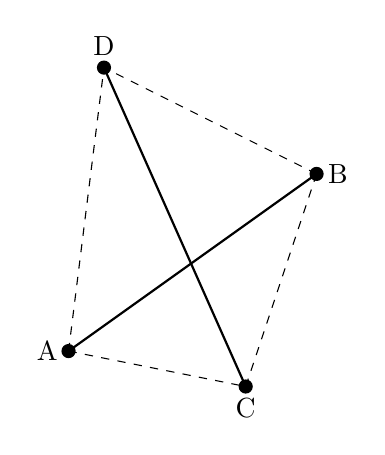
\begin{tikzpicture}[scale=0.9]
\draw[thick, circle] (0, 0.5) -- (3.5,3);
\draw[thick, circle] (2.5, 0) -- (0.5,4.5);
\fill[black] (0, 0.5) circle (0.1);
\fill[black] (3.5,3) circle (0.1);
\fill[black] ((2.5, 0) circle (0.1);
\fill[black] (0.5,4.5) circle (0.1);
\draw[dashed] (0, 0.5) -- (0.5,4.5);
\draw[dashed] (0, 0.5) -- (2.5, 0);
\draw[dashed] (2.5, 0) -- (3.5,3);
\draw[dashed] (3.5,3) -- (0.5,4.5);
\draw (-0.3,0.5) node{A};
\draw (3.8,3) node{B};
\draw(2.5, -0.3) node{C};
\draw (0.5,4.8) node{D};
\end{tikzpicture}
\caption{Intersecting line segments}
\label{segments}
\end{figure}